\chapter{Data Engineering for LLM Applications}
\label{ch:data-engineering}

\noindent
There's an uncomfortable truth that the AI industry prefers not to advertise: for most production LLM applications, the data engineering work---building and maintaining the data pipelines that feed context to the model---is two to three times harder than the actual LLM integration. A RAG pipeline that works beautifully on your demo dataset of 50 clean markdown files will collapse spectacularly when pointed at your company's actual knowledge base: 30,000 PDFs (half of them scanned images), a Confluence wiki with 8 years of accumulated cruft, Slack messages that mix code snippets with emoji reactions, and a Jira backlog where the same bug has been filed 17 times with 17 different descriptions.

This chapter covers the data engineering challenges specific to LLM applications: document processing, embedding pipelines, vector database operations, and the ongoing maintenance that keeps your data layer healthy over time.

\begin{figure}[htbp]
\centering
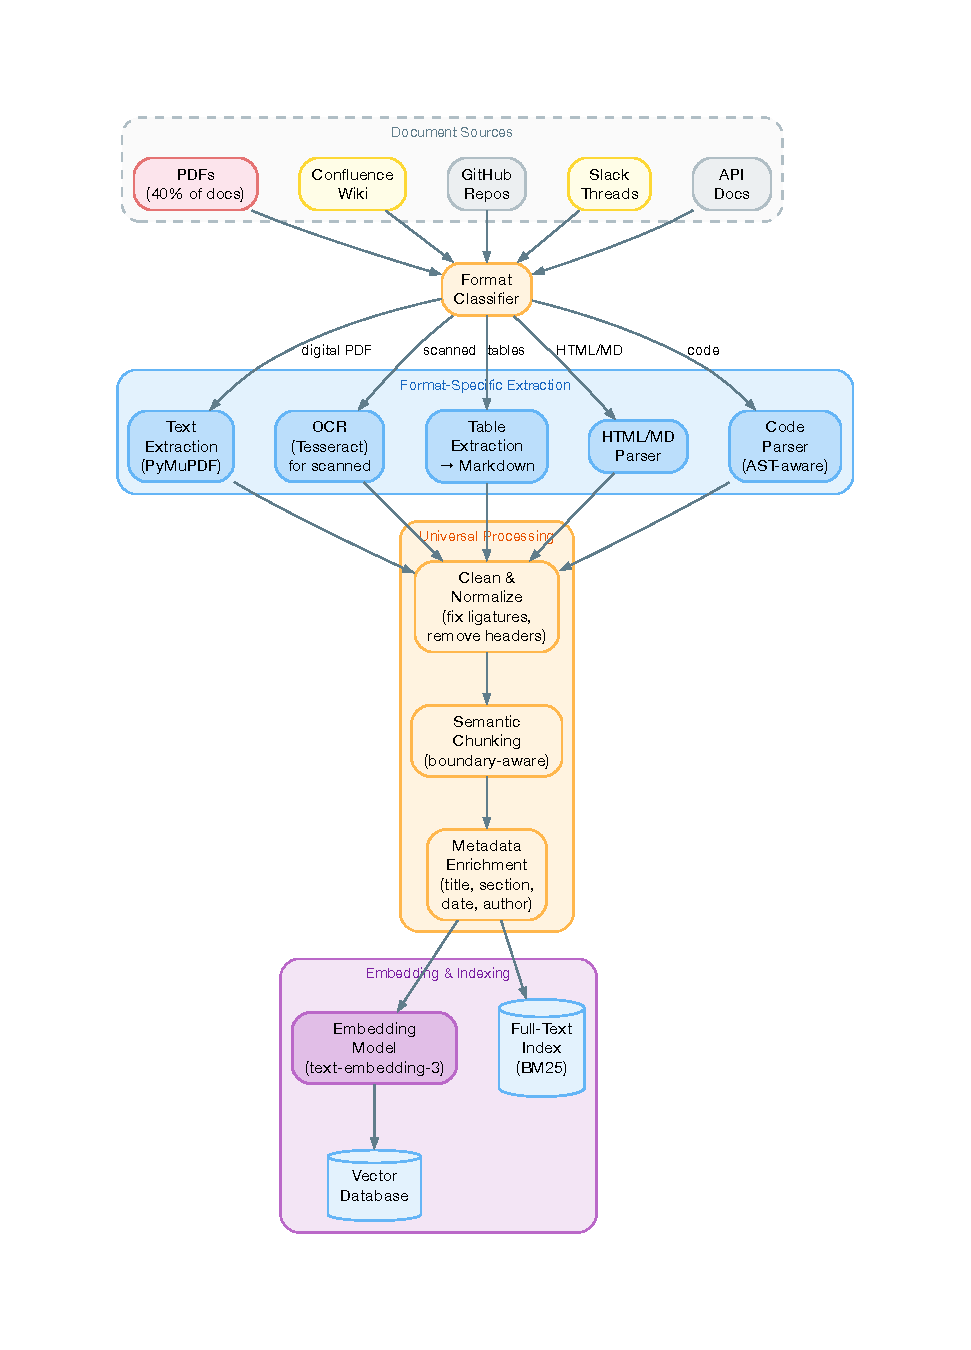
\includegraphics[width=\textwidth]{diagrams/compiled/ch07/document-processing-pipeline.pdf}
\caption{The document processing pipeline: heterogeneous sources → format-specific extraction → universal processing → dual indexing}
\label{fig:doc-pipeline}
\end{figure}


\section{The Document Processing Pipeline}

The first challenge in any RAG system is getting documents into a format the LLM can use. This sounds trivial until you encounter the diversity of real enterprise document formats.

\subsection{The Dirty Truth About PDFs}

PDFs are the bane of every RAG system. They are not designed for text extraction---they are designed for visual rendering. A ``simple'' PDF extraction pipeline must handle:

\begin{lstlisting}[language=Python, caption={Production PDF processing: the reality}]
from dataclasses import dataclass, field
from enum import Enum

class PDFComplexity(Enum):
    SIMPLE_TEXT = "simple_text"       # Born-digital, single column
    MULTI_COLUMN = "multi_column"     # Academic papers, reports
    TABLES = "tables"                 # Financial statements, specs
    SCANNED = "scanned"              # Literally an image of text
    MIXED = "mixed"                  # All of the above in one doc

@dataclass
class PDFProcessor:
    """
    Production PDF processor. The complexity here is NOT the LLM
    integration -- it's handling the 15 different ways a PDF
    can store text.
    
    Real stats from a legal firm migration:
    - 40% simple text (PyMuPDF handles fine)
    - 25% multi-column (need layout analysis)
    - 20% tables (need table extraction)  
    - 10% scanned (need OCR)
    - 5% mixed (need all of the above)
    """
    def process(self, pdf_path: str) -> list[DocumentChunk]:
        complexity = self._classify_pdf(pdf_path)
        
        if complexity == PDFComplexity.SIMPLE_TEXT:
            text = self._extract_with_pymupdf(pdf_path)
        elif complexity == PDFComplexity.SCANNED:
            text = self._ocr_with_tesseract(pdf_path)
        elif complexity == PDFComplexity.TABLES:
            # Tables need special handling: extract as structured
            # data, then convert to markdown tables for the LLM
            text = self._extract_tables(pdf_path)
        else:
            # Multi-column and mixed: use layout-aware extraction
            text = self._layout_aware_extract(pdf_path)
        
        # Universal post-processing
        text = self._fix_common_issues(text)
        return self._chunk(text)
    
    def _fix_common_issues(self, text: str) -> str:
        """The things nobody warns you about."""
        # Fix hyphenation from line breaks ("impor-\ntant")
        text = re.sub(r'(\w)-\n(\w)', r'\1\2', text)
        # Fix ligatures (fi -> fi, fl -> fl)
        text = text.replace('fi', 'fi').replace('fl', 'fl')
        # Remove page headers/footers (heuristic)
        text = self._remove_repeated_headers(text)
        # Normalize whitespace
        text = re.sub(r'\n{3,}', '\n\n', text)
        return text
\end{lstlisting}

\subsection{Chunking Strategies}

Chunking---splitting documents into pieces for retrieval---is where most RAG pipelines quietly fail. The wrong chunking strategy means the most relevant information is split across two chunks, and neither one has enough context to be useful.

\begin{lstlisting}[language=Python, caption={Semantic chunking: split at meaning boundaries, not character counts}]
class SemanticChunker:
    """
    Chunks documents at natural semantic boundaries rather
    than at fixed character counts.
    
    The difference matters: fixed-size chunking splits a
    function definition in half. Semantic chunking keeps
    it together.
    """
    def __init__(self, 
                 embedding_model,
                 max_chunk_tokens: int = 512,
                 similarity_threshold: float = 0.5):
        self.embedder = embedding_model
        self.max_tokens = max_chunk_tokens
        self.threshold = similarity_threshold
    
    def chunk(self, text: str) -> list[str]:
        # Step 1: Split into sentences
        sentences = self._split_sentences(text)
        
        # Step 2: Compute embeddings for each sentence
        embeddings = self.embedder.encode(sentences)
        
        # Step 3: Find natural break points
        chunks = []
        current_chunk = [sentences[0]]
        
        for i in range(1, len(sentences)):
            # Compare this sentence to the current chunk's centroid
            similarity = cosine_similarity(
                embeddings[i],
                np.mean([embeddings[j] for j in 
                        range(len(current_chunk))], axis=0)
            )
            
            chunk_text = " ".join(current_chunk + [sentences[i]])
            token_count = self._count_tokens(chunk_text)
            
            if similarity < self.threshold or \
               token_count > self.max_tokens:
                # Semantic break: start new chunk
                chunks.append(" ".join(current_chunk))
                current_chunk = [sentences[i]]
            else:
                current_chunk.append(sentences[i])
        
        if current_chunk:
            chunks.append(" ".join(current_chunk))
        
        return chunks
\end{lstlisting}

\begin{tipbox}[Chunking Rules of Thumb]
After working with dozens of RAG systems, these rules consistently produce better retrieval quality:
\begin{enumerate}
    \item \textbf{Chunk code differently than prose}: Code should be chunked at function/class boundaries, not by token count
    \item \textbf{Include overlapping context}: 10--15\% overlap between adjacent chunks prevents information loss at boundaries
    \item \textbf{Add metadata headers}: Prepend each chunk with its source document title, section heading, and page number
    \item \textbf{Don't chunk too small}: Chunks under 100 tokens lack sufficient context for meaningful retrieval
    \item \textbf{Don't chunk too large}: Chunks over 1024 tokens dilute the semantic signal and waste context window
\end{enumerate}
\end{tipbox}

\section{Embedding Pipelines at Scale}

Computing embeddings for a large document corpus is a batch processing problem with specific engineering challenges.

\begin{lstlisting}[language=Python, caption={Production embedding pipeline with incremental updates}]
class EmbeddingPipeline:
    """
    Manages the embedding of documents at scale.
    Key challenge: keeping the index up-to-date as 
    documents are added, modified, and deleted.
    """
    def __init__(self, 
                 embedding_model: str = "text-embedding-3-small",
                 vector_store: VectorStore = None,
                 batch_size: int = 100):
        self.model = embedding_model
        self.store = vector_store
        self.batch_size = batch_size
    
    def full_index(self, documents: list[Document]):
        """Initial indexing of all documents."""
        for batch in self._batch(documents, self.batch_size):
            chunks = []
            for doc in batch:
                doc_chunks = self.chunker.chunk(doc.text)
                for i, chunk_text in enumerate(doc_chunks):
                    chunks.append(Chunk(
                        text=chunk_text,
                        metadata={
                            "source": doc.source,
                            "doc_id": doc.id,
                            "chunk_index": i,
                            "content_hash": hashlib.md5(
                                chunk_text.encode()
                            ).hexdigest(),
                            "indexed_at": datetime.utcnow().isoformat(),
                        }
                    ))
            
            embeddings = self._embed_batch(
                [c.text for c in chunks]
            )
            self.store.upsert(chunks, embeddings)
    
    def incremental_update(self, changed_docs: list[Document]):
        """
        Only re-embed documents that have actually changed.
        Uses content hashing to avoid unnecessary API calls.
        
        This saves 60-80% of embedding costs for 
        documentation that updates daily.
        """
        for doc in changed_docs:
            new_chunks = self.chunker.chunk(doc.text)
            existing = self.store.get_by_doc_id(doc.id)
            
            # Compare content hashes
            new_hashes = {
                hashlib.md5(c.encode()).hexdigest() 
                for c in new_chunks
            }
            old_hashes = {
                c.metadata["content_hash"] for c in existing
            }
            
            if new_hashes == old_hashes:
                continue  # Nothing changed, skip
            
            # Something changed: delete old, embed new
            self.store.delete_by_doc_id(doc.id)
            self._embed_and_store(doc, new_chunks)
\end{lstlisting}

\section{Vector Database Operations}

\subsection{Choosing the Right Vector Database}

\begin{table}[htbp]
\centering
\caption{Vector database comparison for LLM applications}
\label{tab:vector-dbs}
\begin{tabularx}{\textwidth}{lXXX}
\toprule
\textbf{Database} & \textbf{Best For} & \textbf{Latency (p99)} & \textbf{Key Trade-off} \\
\midrule
pgvector & Teams already on PostgreSQL; small-medium datasets (< 5M vectors) & 10--50ms & Easy adoption, limited scale \\
Pinecone & Managed service, fast setup; no infrastructure team & 5--20ms & Vendor lock-in, cost at scale \\
Weaviate & Hybrid search (dense + sparse), multi-tenancy & 10--40ms & Complex config, heavier infra \\
Qdrant & On-prem, large datasets, payload filtering & 5--30ms & More operational overhead \\
ChromaDB & Prototyping, local development & N/A (local) & Not for production \\
\bottomrule
\end{tabularx}
\end{table}

\begin{cautionbox}[The pgvector Trap]
pgvector is the most common first choice because ``we already have Postgres.'' This works fine for datasets under 1 million vectors. Beyond that, pgvector's HNSW index struggles: queries slow down, memory usage spikes, and VACUUM operations become painfully long. Plan your migration path before you hit this wall.
\end{cautionbox}

\section{Data Quality Monitoring}

The hardest part of data engineering for LLMs isn't building the pipeline---it's maintaining it. Data quality degrades silently, and by the time users notice, the damage is done.

\begin{lstlisting}[language=Python, caption={Continuous data quality monitoring}]
class DataQualityMonitor:
    """
    Runs daily to detect data quality regressions.
    Inspired by the approach used at Notion for their
    AI knowledge base features.
    """
    def daily_check(self) -> QualityReport:
        issues = []
        
        # 1. Freshness: are we actually indexing new documents?
        latest = self.store.get_most_recent()
        age = datetime.utcnow() - latest.metadata["indexed_at"]
        if age > timedelta(hours=24):
            issues.append(Issue(
                severity="high",
                message=f"Index stale: last update {age.hours}h ago",
            ))
        
        # 2. Completeness: spot-check that known docs exist
        for canary_doc in self.canary_documents:
            results = self.store.search(canary_doc.title, top_k=1)
            if not results or results[0].score < 0.8:
                issues.append(Issue(
                    severity="critical",
                    message=f"Canary doc missing: {canary_doc.title}",
                ))
        
        # 3. Quality: sample random chunks, check for corruption
        sample = self.store.random_sample(n=100)
        for chunk in sample:
            if len(chunk.text.strip()) < 50:
                issues.append(Issue(
                    severity="medium",
                    message=f"Empty/short chunk: {chunk.id}",
                ))
            if chunk.text.count('\x00') > 0:
                issues.append(Issue(
                    severity="high",
                    message=f"Null bytes in chunk: {chunk.id}",
                ))
        
        return QualityReport(issues=issues, checked_at=datetime.utcnow())
\end{lstlisting}

\section{Chapter Summary}

Data engineering for LLM applications is the unglamorous work that determines whether your AI features actually work:

\begin{enumerate}[leftmargin=*]
    \item \textbf{Document processing is 80\% of the work}: PDFs, Confluence, Slack, Jira---each format has unique extraction challenges
    \item \textbf{Chunking strategy determines retrieval quality}: Semantic chunking outperforms fixed-size chunking, but requires more engineering
    \item \textbf{Incremental indexing saves money}: Content-hash-based updates reduce embedding API costs by 60--80\%
    \item \textbf{Choose your vector database based on scale}: pgvector for $<$1M vectors, purpose-built databases for larger datasets
    \item \textbf{Monitor data quality continuously}: Canary documents, freshness checks, and sample-based validation catch silent degradation
\end{enumerate}
